\section{Spine segmentation}

\subsection{Loss functions}
One of the most important things to get good results with neural networks is to choose a suitable loss function. Loss function measures how well the network's predictions are during training. The goal of the network is to minimise its value. Some of them lead to convergence of the network, some of them do not.

There are numerous loss functions used for image segmentation. Since my data is very unbalanced, some losses were more suitable than the others. Badly chosen loss with unbalanced data can lead to predicting only zeros (only background). I chose 2 and compared their performance.

One of the losses that perform well on unbalanced data is Dice loss. It is an overlap measure. Instead of evaluating every pixel (voxel) independently, Dice looks at how well the ground truth and the prediction overlap. This means that if half of a small object and half of a large object are detected, the loss will be the same.

Another loss function I used is binary crossentropy. To put it simply, a negative logarithm for every prediction is computed. This means that if the prediction for the object pixel is 1, loss will be also 1. And similarly, for very low predictions logarithm gets bigger and bigger. This loss on itself does not deal with class imbalance. For this reason I computed class weights and multiplied the crossentropy results by them, making the spine object ``more important'' than the background. By using this loss I tried to solve the gradient exploding and instability issues I encountered with Dice loss - I can say they did not occur with binary crossentropy.

\subsection{Training}
The size of the dataset is 80 scans. The data was split in the ratio of 80/10/10, which means 64 scans were used for training, 8 for validation and 8 for testing. The data was sorted in the same order as it was originally in the dataset, no special selection of the split. I chose this ratio, as the dataset is rather small and I wanted to reserve as many examples for training as I could. The algorithm ran on a Cloud TPU with 35GB RAM offered by Google Colab. Models were trained for 40 epochs, which took approximately 10 hours. 

I will be comparing 2 models, one trained with binary crossentropy loss (Model 1) and Dice loss (Model 2). Both were trained with stochastic gradient descent - this means the batch size was 1 and weights were updated for each example of the training set. This approach proved to be considerably faster than the mini-batch approach (8 batches). Input images were normalised to the range (0,1). 

Model 1 was trained with Adam optimizer, \textit{learning\_rate}=0.0001, \textit{beta\_1 = 0.9}, \textit{beta\_2 = 0.999}. Choosing parameters for Model 2 with Dice loss was more difficult, exploding gradients occurred frequently. Learning rates for Adam optimizer I tried include: 0.001, 0.00015, 0.0001, 0.000015, 0.00001 and 0.000001. I settled for \textit{learning\_rate} = 0.00001 together with clip\_norm = 1. and clip\_value = 0.5 (to prevent exploding/vanishing gradients) as it was one of the few settings to yield reasonable results. \textit{beta\_1 = 0.9} and \textit{beta\_2 = 0.999} are the same as with Model 1.

\subsection{Metrics}
Often it is difficult to choose the metric that best represents how good our results are. Therefore I chose 4 different metrics, where each of them takes into account different things. In the following equations, \textit{TP} stands for true positive, \textit{TN} for true negative, \textit{FP} for false positive and \textit{FN} for false negatives.

Pixel wise accuracy (Eq. \ref{eq:pixel-wise-accuracy}) is a metric that simply measures the percentage of correctly classed pixels. However, this metric gives good results also for images with very small objects, even though they are not classified properly.

\begin{equation}
\label{eq:pixel-wise-accuracy}
    \textup{pixel wise accuracy}  = \frac{TP + TN}{TP + TN + FP + FN} 
\end{equation}

Dice coefficient (Eq. \ref{eq:dice-accuracy}) was explained before. It measures overlap between the ground truth and predicted object. 

\begin{equation}
\label{eq:dice-accuracy}
    \textup{dice coefficient}  = \frac{2TP}{2TP + FP + FN} = \frac{2|X\cap Y|}{|X|+|Y|}
\end{equation}

Intersction over Union (IoU) (Eq. \ref{eq:iou-accuracy}) is very similar to Dice. It measures overlap as well, but penalizes wrong predictions more than Dice. 

\begin{equation}
\label{eq:iou-accuracy}
    \textup{IoU}  = \frac{TP}{TP + FP + FN} = \frac{2|X\cap Y|}{|X|+|Y| - |X\cap Y|}
\end{equation}

The last metric AUC-ROC Curve (Area under Curve - Receiver Operating Characteristics curve) is a metric that measures how well the model can separate classes. Value 0.5 means it cannot distinguish between classes at all.   

\subsection{Results}
Results for all 4 metrics for Model 1 and Model 2 are in Table \ref{tab:results-spine}. Predictions were thresholded at 0.9. Model 2 performed significantly better in all metrics except for AUC-ROC, which means it is worse at separating classes. 

Sample predictions and segmentations are in Fig. \ref{fig:spine-segmentations} and more in the appendix. We can see that predictions with Model 2 (with Dice loss) are very tightly around the spine, have smooth edges. There are a lot of false negatives, as the model seems to be trying to not class background as foreground. Model 1 (with weigthed binary crossentropy), on the other hand, is able to spot more details and irregularities. However, for the price of false positives, when it often detects areas outside of the object. The weighted binary crossentropy ensured that pixels are not easily classed as the background.

For cross validation and comparison with another architecture, I chose Model 2 (or rather its hyper-parameters and validation loss), as it outperformed Model 1 in almost all metrics. Furthermore, as you can see in Fig. \ref{fig:spine-losses}, performance of Model 2 was consistently getting better, while Model 1 seemed to have reached its best at around the 20th epoch, with validation loss not getting much better since. It was only train loss which was decreasing, meaning the model was overfit.  

\begin{figure}
\begin{subfigure}{.5\textwidth}
  \centering
  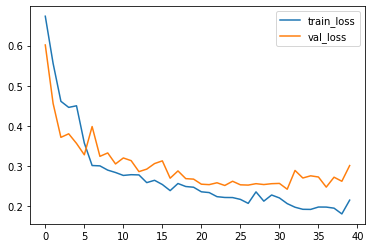
\includegraphics[width=.8\linewidth]{images/loss-binary.png}
  \caption{Model 1}
  \label{fig:sfig1}
\end{subfigure}%
\begin{subfigure}{.5\textwidth}
  \centering
  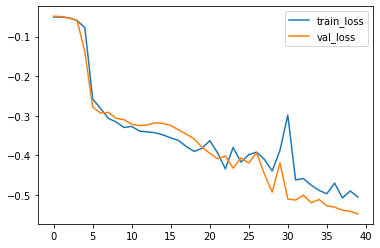
\includegraphics[width=.8\linewidth]{images/loss-dice.png}
  \caption{Model 2}
  \label{fig:sfig2}
\end{subfigure}
\caption[Loss over epochs for Model 1 and 2]{Validation and training loss over 40 epochs for Model 1 and 2. X axis represents number of epochs, Y axis is loss.}
\label{fig:spine-losses}
\end{figure}


To ensure generalisation, I performed 3-fold cross validation on 72 samples. Since training the network is very time consuming, I decided to cross validate the network only on 20 epochs. The folds were chosen randomly. Results, again for all four metrics, are in \ref{tab:cross-val-spine}. Even after only 20 epochs, the results are generally better than for Model 1 after 40 epochs. Small standard deviations also suggest, that accuracy did not change much across the folds.


The idea behind my architecture is that 3D convolutions should be better at  extracting features from 3D volumes, because they can ``capture'' the third dimension. Therefore, I compared my model with the corresponding 2D one. The input were 96x96 axial slices of the spine. Hyper-parameters and validation loss for training were the same as for Model 2, except for the batch size, which I set to 32, which is a widely used value. The number of epochs was 40 and the training took only 3.5 hours. Results are in Table \ref{tab:results-spine-2D}. Both the models yielded similar results, with UNet 2D being slightly better, but not significantly. Comparison of segmentations is in Fig. \ref{fig:unet2D-spine}. UNet 2D was able to capture more details and edges than UNet 3D. 





%-------------------------------------------------------------------

\begin{figure}[ht!]
\centering
\begin{subfigure}[b]{0.70\textwidth}
   \includegraphics[width=1\linewidth]{images/results_1/original.png}
   \caption{Original image}
   \label{fig:Ng1} 
\end{subfigure}

\begin{subfigure}[b]{0.70\textwidth}
   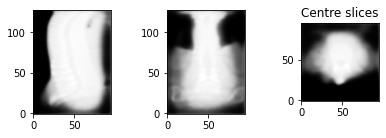
\includegraphics[width=1\linewidth]{images/results_1/binary_mask.png}
   \caption{Predictions of Model 1}
   \label{fig:Ng2}
\end{subfigure}

\begin{subfigure}[b]{0.70\textwidth}
   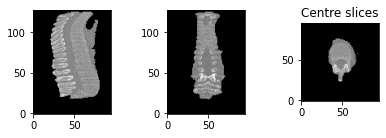
\includegraphics[width=1\linewidth]{images/results_1/binary_segmented.png}
   \caption{Segmented image with Model 1}
   \label{fig:Ng3}
\end{subfigure}

\begin{subfigure}[b]{0.70\textwidth}
   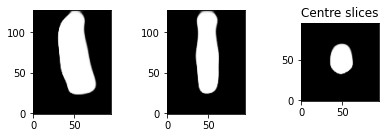
\includegraphics[width=1\linewidth]{images/results_1/dice_mask.png}
   \caption{Predictions of Model 2}
   \label{fig:Ng4}
\end{subfigure}

\begin{subfigure}[b]{0.70\textwidth}
   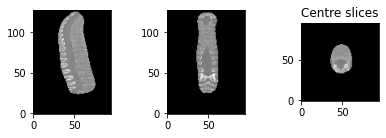
\includegraphics[width=1\linewidth]{images/results_1/dice_segmented.png}
   \caption{Segmented image with Model 2}
   \label{fig:Ng5}
\end{subfigure}

\caption[Results of spine segmentation]{Original and segmented CT image of a spine using Model 1 and Model 2.}
\label{fig:spine-segmentations}
\end{figure}

%---------------------------------------------------------------

\begin{table}[ht!]
\centering
\begin{tabular}{@{}ccc@{}}
\toprule
Metric                  & Model 1    & Model 2   \\ \midrule
Pixel wise accuracy     & 0.90773034 & 0.9738508 \\
Dice coefficient        & 0.36018768 & 0.6070875 \\
Intersection over union & 0.21965213 & 0.435841  \\
Area under ROC          & 0.9219055  & 0.8547937 \\ \bottomrule
\end{tabular}
\caption[Comparison of Model 1 and 2]{Comparison of Model 1 and Model 2. Metrics used: pixel wise accuracy, Dice coefficient, intersection over union and area under ROC}
\label{tab:results-spine}
\end{table}

%---------------------------------------------------------------

\begin{table}[ht!]
\centering
\begin{tabular}{@{}cc@{}}
\toprule
Metric                  & 3D UNet                 \\ \midrule
Pixel wise accuracy     & 0.959435(+/- 0.010288)  \\
Dice coefficient        & 0.397100 (+/- 0.008332) \\
Intersection over union & 0.247772 (+/- 0.006509) \\
Area under ROC          & 0.730441 (+/- 0.038218) \\ \bottomrule
\end{tabular}
\caption[3-fold Cross validation] {Results of 3-fold cross validation after 20 epochs with 3D UNet, standard deviation included. Evaluated with 4 different metrics: pixel wise accuracy, Dice coefficient, intersection over union and area under ROC}
\label{tab:cross-val-spine}
\end{table}

%---------------------------------------------------------------

\begin{figure}[ht!]
\centering
\begin{subfigure}[b]{0.70\textwidth}
   \includegraphics[width=1\linewidth]{images/results_3/original.png}
   \caption{Original image}
   \label{fig:Ng1} 
\end{subfigure}

\begin{subfigure}[b]{0.70\textwidth}
   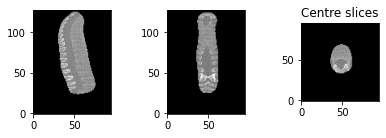
\includegraphics[width=1\linewidth]{images/results_3/3D.png}
   \caption{Segmented image with 3D UNet}
   \label{fig:Ng2}
\end{subfigure}

\begin{subfigure}[b]{0.70\textwidth}
   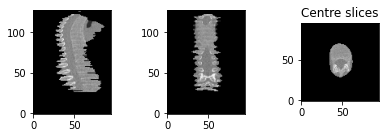
\includegraphics[width=1\linewidth]{images/results_3/2D.png}
   \caption{Segmented image with 2D UNet}
   \label{fig:Ng3}
\end{subfigure}

\caption[Comparison UNet 3D and UNet 2D]{Original and segmented CT image of a spine using Model 1 and Model 2. Threshold for predictions is 0.9.}
\label{fig:unet2D-spine}
\end{figure}

%---------------------------------------------------------------

\begin{table}[ht!]
\centering
\begin{tabular}{@{}ccc@{}}
\toprule
Metric                  & UNet 2D    & UNet 3D   \\ \midrule
Pixel wise accuracy     & 0.97514015 & 0.9738508 \\
Dice coefficient        & 0.6125695 & 0.6070875 \\
Intersection over union & 0.44151428 & 0.435841  \\
Area under ROC          & 0.8458461  & 0.8547937 \\ \bottomrule
\end{tabular}
\caption[UNet 2D and UNet 3D results]{Comparison of results from 3D and 2D UNet using metrics: pixel wise accuracy, Dice coefficient, intersection over union and area under ROC}
\label{tab:results-spine-2D}
\end{table}

\subsection{Summary}
I managed to get good results with the 3D UNet network. The spine is correctly located in the images. However, still unable to detect space inbetween vertebrae. There is a potential to improve performance by training the model for more epochs, because the loss was still steadily improving. Cross validation results proved the model can generalise well for the given dataset. However, the 3D architecture did not bring any improvement compared to the 2D one, as the results were very similar, with 2D one slightly outperforming the 3D one. 